\chapter{Zusammenfassung}
In dieser Arbeit wurde die Amplitude der \CP-Asymmetrie $\SJPsi$ gemessen. Es wurde dabei die sFit-Methode angewandt, um Signal vom Untergund zu extrahieren. Dazu diente ein Fit der rekonstruierten \Bd-Masse. Aus dem anschließenden Fit der Eigenzeitverteilung erhält man
\begin{align}
\SJPsi = \sin(2\beta) = 0,711 \pm 0,059 (\text{stat.}) \pm 0,033 (\text{syst.})
\end{align}
Hierbei soll erwähnt werden, dass der statistische Fehler auf Grund der Erkenntnisse aus Kapitel \ref{kap:fit_bias} um den Faktor $\sigma_{\text{pull}} = 0,941$ korrigiert wurde. Das Ergebnis ist kompatibel zum Weltmittelwert $\sin(2\beta) = 0,682 \pm 0,019$ \cite{pdg-average} sowie zur LHCb-Analyse aus 2011 $\sin(2\beta) = 0.72 \pm 0,07 (\text{stat.}) \pm 0,04 (\text{syst.})$ \cite{lhcb-paper}. 

\begin{figure}[hptb]
\centering
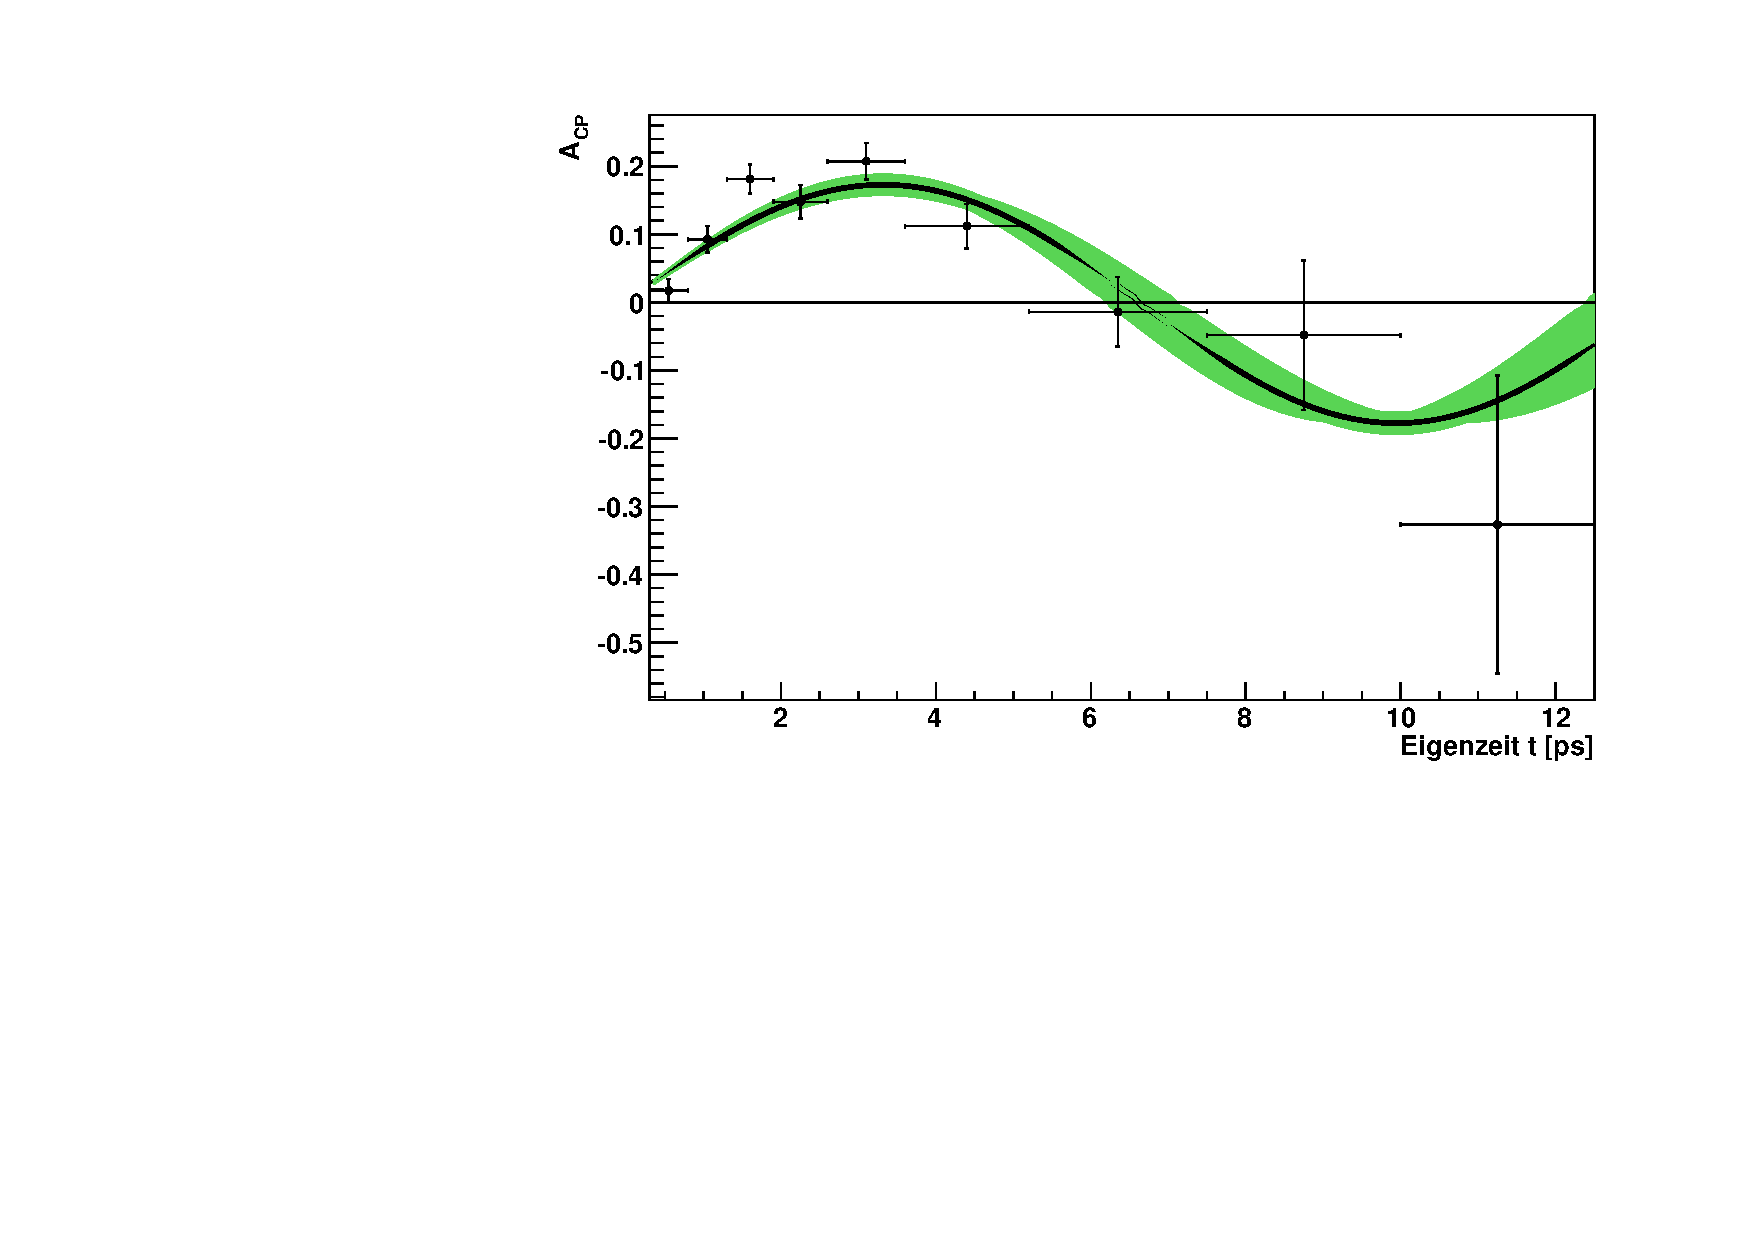
\includegraphics[width=\textwidth]{asymmetrie}
\caption{Darstellung der \CP-Asymmetrie $\mathcal{A_{CP}}$ nach Definition aus Gleichung \ref{eq:cp_asymm_def}. Für die dazugehörige Kurve wurden die aus dem Eigenzeitfit erhaltenen Parameter in Gleichung (\ref{eq:cp_asymm_meas}) eingesetzt. Das grüne Band entspricht den $1\sigma^{\text{stat.}}$ Abweichungen von $\SJPsi$ und $\Delta m_d$.}
\label{fig:asymmetrie}
\end{figure}

Abbildung \ref{fig:asymmetrie} zeigt die \CP-Asymmetrie des Signals. Die Messung von $\sin(2\beta)$ bzw. $\Delta\SJPsi$ könnte wie folgt modifiziert werden:
\begin{enumerate}
    \item Bei der Erstellung des NTupels kann die neueste Version der Analysesoftware verwendet werden, bei der die Wahrscheinlichkeit, dass es sich bei den Pionspuren um Phantome handelt, richtig kalibriert ist. Dies würde ermöglichen, bereits vor dem Fit den Datensatz etwas besser von Untergrund zu bereinigen.
    \item Als dominierende Systematik sollte der Einfluss der Kalibration der Flavour Tagging Algorithmen auf $\SJPsi$ erneut bestimmt werden, sobald die systematischen Studien des hier verwendeten Flavour Taggings abgeschlossen sind.
    \item Sobald der LHC wieder in Betrieb geht, werden mit fortlaufender Betriebsdauer mehr Daten zur Verfügung stehen, die die statistische Präzision erhöhen. Diese Analyse konnte zeigen, dass hier noch Potential besteht, da die statistische Unsicherheit etwa doppelt so groß wie die systematische ist.
\end{enumerate}
